% ============================================================
%  Math Mirror: A Self-Validating Byte-Level Transformer
%  for Agentic Mathematics
%
%  Author: Jianghan Zhang, Dartmouth College
%  Target: arXiv math.ML
% ============================================================
\documentclass[11pt,a4paper]{article}

% ── Packages (minimal set) ──────────────────────────────────
\usepackage[utf8]{inputenc}
\usepackage[T1]{fontenc}
\usepackage{amsmath,amssymb,amsthm}
\usepackage{mathtools}
\usepackage{enumitem}
\usepackage{booktabs}
\usepackage{hyperref}
\usepackage[margin=1in]{geometry}
\usepackage{algorithm}
\usepackage{algpseudocode}
\usepackage{tikz}
\usetikzlibrary{arrows.meta,positioning,calc}

% ── Theorem environments ────────────────────────────────────
\newtheorem{theorem}{Theorem}[section]
\newtheorem{proposition}[theorem]{Proposition}
\newtheorem{lemma}[theorem]{Lemma}
\newtheorem{corollary}[theorem]{Corollary}
\newtheorem{definition}[theorem]{Definition}
\newtheorem{remark}[theorem]{Remark}
\newtheorem{example}[theorem]{Example}

% ── Notation ────────────────────────────────────────────────
\newcommand{\R}{\mathbb{R}}
\newcommand{\Z}{\mathbb{Z}}
\newcommand{\N}{\mathbb{N}}
\newcommand{\cM}{\mathcal{M}}
\newcommand{\cV}{\mathcal{V}}
\newcommand{\cD}{\mathcal{D}}
\newcommand{\cL}{\mathcal{L}}
\newcommand{\cF}{\mathcal{F}}
\newcommand{\cG}{\mathcal{G}}
\newcommand{\cS}{\mathcal{S}}
\newcommand{\cT}{\mathcal{T}}
\newcommand{\cB}{\mathcal{B}}
\newcommand{\cA}{\mathcal{A}}
\newcommand{\cX}{\mathcal{X}}
\newcommand{\cP}{\mathcal{P}}
\newcommand{\cE}{\mathcal{E}}
\newcommand{\ip}[2]{\langle #1, #2 \rangle}
\newcommand{\norm}[1]{\lVert #1 \rVert}
\newcommand{\abs}[1]{\lvert #1 \rvert}
\newcommand{\DKL}{D_{\mathrm{KL}}}
\newcommand{\Breg}{D_\psi}
\newcommand{\softmax}{\mathrm{softmax}}
\newcommand{\Verify}{\mathrm{Verify}}
\newcommand{\Embed}{\mathrm{Embed}}
\newcommand{\Pullback}{\mathrm{Pullback}}
\newcommand{\Mirror}{\mathrm{Mirror}}
\newcommand{\ASCII}{\mathrm{ASCII}}

% ============================================================
\title{\textbf{Math Mirror: A Self-Validating Byte-Level Transformer\\
for Agentic Mathematics}}

\author{Jianghan Zhang\\
Department of Computer Science\\
Dartmouth College\\
\texttt{jianghan.zhang.gr@dartmouth.edu}}

\date{February 2026}

\begin{document}
\maketitle

% ============================================================
%  Abstract
% ============================================================
\begin{abstract}
We present \emph{Math Mirror}, a byte-level transformer architecture
trained exclusively on self-validated mathematical data.
The model operates over a vocabulary of 256 ASCII characters,
eliminating hidden tokenization and ensuring that the model's
internal representation is identical to the user-visible output.
Every training example is generated by symbolic computation
(SymPy) and verified before inclusion in the dataset,
guaranteeing that no mathematically incorrect statement
enters the training distribution.
At inference time, a three-level symbolic verification gate
rejects any output that cannot be confirmed correct.
We formalize the \emph{embed-prove-pullback} architecture,
in which a large language model (LLM) translates natural language
to mathematical ASCII at the boundary, the mirror computes
in pure mathematical space, and verified results return through
the LLM for human-readable presentation.
Finetuning is explicit and opt-in only: the model never learns
from conversations, preserving privacy by architecture.
We establish formal connections to the renormalization group (RG)
through mirror descent, and to the agent-nucleation framework
through the $V(T,B)$ protocol.
The core thesis is that a model trained only on verified mathematics
is sufficient for mathematical reasoning within its verified domain,
and that self-validation eliminates hallucination by construction.
\end{abstract}

\tableofcontents

% ============================================================
%  Section 1: Introduction
% ============================================================
\section{Introduction}\label{sec:intro}

Large language models (LLMs) achieve remarkable performance across
diverse tasks, yet they suffer from a fundamental limitation in
mathematical reasoning: \emph{hallucination}~\cite{Ji2023}.
An LLM can fluently produce mathematical text that is syntactically
correct but semantically wrong---an integral with the wrong sign,
a proof with a gap, an identity that fails at a single point.
The problem is structural: LLMs are trained on natural language
corpora where mathematical content is a small fraction,
and the training objective (next-token prediction) does not
distinguish correct mathematics from plausible-looking mathematics.

We propose a different approach.
Instead of training a large model on everything and hoping
it learns mathematics as a side effect, we train a small model
on \emph{nothing but mathematics}, and we verify every training
example and every output.

\subsection{Three design principles}

\begin{enumerate}[label=(\roman*),nosep]
\item \textbf{Self-validation.}
  Mathematics is the unique domain where correctness can be
  checked mechanically.
  The identity $\sin^2 x + \cos^2 x = 1$ needs no human label;
  a computer algebra system can verify it.
  We exploit this by generating all training data through
  symbolic computation and verifying every example before
  it enters the dataset.

\item \textbf{Transparency.}
  Standard LLM tokenizers (BPE, SentencePiece) create a hidden
  layer between the model's internal representation and
  the user-visible text.
  The token \texttt{" math"} with a leading space is different
  from \texttt{"math"} without one, but the user cannot see
  this distinction.
  We eliminate this problem entirely by using a byte-level
  vocabulary: $|\cV| = 256$, one token per ASCII character.
  What the model sees \emph{is} what the user sees.

\item \textbf{Architectural separation.}
  The mirror model is not an LLM.
  It does not generate natural language.
  An LLM serves as the \emph{boundary translator}:
  it converts natural language to mathematical ASCII (embed)
  and converts verified mathematical output back to natural
  language (pullback).
  The mirror operates entirely in mathematical space.
\end{enumerate}

\subsection{Contributions}

\begin{enumerate}[nosep]
\item A formal specification of the \emph{Math Mirror} architecture:
  a byte-level transformer ($|\cV| = 256$, $d = 256$,
  $L = 12$ layers, $H = 8$ heads) trained on self-validated
  mathematical data (\S\ref{sec:arch}).

\item A self-validated training pipeline
  that generates and verifies training data using symbolic
  computation, with no human labels (\S\ref{sec:training}).

\item A three-level verification gate
  (well-formedness, identity checking, derivation verification)
  that rejects unverified outputs at inference time (\S\ref{sec:gate}).

\item The \emph{embed-prove-pullback} protocol
  for agentic mathematics, with formal boundary conditions
  between the LLM and the mirror (\S\ref{sec:mirror}).

\item An explicit finetuning protocol
  that updates model weights only from user-provided,
  verified examples, with no online learning (\S\ref{sec:finetune}).

\item Formal connections to the renormalization group
  via mirror descent (\S\ref{sec:rg}) and to the
  agent-nucleation framework (\S\ref{sec:agent}).
\end{enumerate}

% ============================================================
%  Section 2: Architecture
% ============================================================
\section{Architecture}\label{sec:arch}

\subsection{The byte-level vocabulary}

\begin{definition}[ASCII vocabulary]\label{def:vocab}
The vocabulary is $\cV = \{0, 1, \ldots, 255\}$,
the standard ASCII character set.
A mathematical expression $e$ is a finite sequence
$e = (v_1, v_2, \ldots, v_T)$ with $v_i \in \cV$ and
$T \leq T_{\max}$, where $T_{\max} = 2048$ is the
context length.
\end{definition}

The choice of ASCII vocabulary is not arbitrary.
It satisfies three desiderata:

\begin{enumerate}[label=(V\arabic*),nosep]
\item \textbf{Transparency:} The mapping between internal tokens
  and displayed characters is the identity.
  There is no hidden tokenization.
\item \textbf{Universality for mathematics:}
  All standard mathematical notation used in computation
  (digits, operators, parentheses, variable names, LaTeX
  control sequences) falls within ASCII.
\item \textbf{Minimality:} $|\cV| = 256 = 2^8$ is the smallest
  vocabulary that satisfies (V1) and (V2).
  This is the minimal lattice for mathematical text.
\end{enumerate}

\subsection{Transformer architecture}

The Math Mirror model is a decoder-only transformer~\cite{Vaswani2017}
with the following specification.

\begin{definition}[Math Mirror transformer]\label{def:model}
The model $\cM_\theta$ is parameterized by:
\begin{itemize}[nosep]
\item Token embedding: $E_{\mathrm{tok}} \in \R^{256 \times d}$
\item Position embedding: $E_{\mathrm{pos}} \in \R^{T_{\max} \times d}$
\item $L$ transformer blocks, each containing:
  \begin{itemize}[nosep]
  \item Multi-head causal self-attention with $H$ heads
  \item Feed-forward network: $\mathrm{FFN}(x) = W_2 \,\sigma(W_1 x + b_1) + b_2$
    where $\sigma$ is GELU and $W_1 \in \R^{4d \times d}$, $W_2 \in \R^{d \times 4d}$
  \item Layer normalization (pre-norm)
  \end{itemize}
\item Output head: $W_{\mathrm{out}} \in \R^{256 \times d}$
\end{itemize}
Default hyperparameters: $d = 256$, $L = 12$, $H = 8$,
$T_{\max} = 2048$.
\end{definition}

The forward pass computes:
\begin{align}
h^{(0)} &= E_{\mathrm{tok}}[v_{1:T}] + E_{\mathrm{pos}}[1{:}T], \label{eq:embed}\\
h^{(\ell)} &= h^{(\ell-1)} + \mathrm{Attn}^{(\ell)}(\mathrm{LN}(h^{(\ell-1)}))
  + \mathrm{FFN}^{(\ell)}(\mathrm{LN}(h^{(\ell-1)} + \mathrm{Attn}^{(\ell)}(\cdots))),
  \label{eq:block}\\
p(v_{T+1} \mid v_{1:T}) &= \softmax(W_{\mathrm{out}} \cdot \mathrm{LN}(h^{(L)}_{T})).
  \label{eq:output}
\end{align}

\begin{remark}[Parameter count]\label{rem:params}
With default hyperparameters, the model has approximately
$12 \times (4 \times 256^2 + 4 \times 256^2) + 2 \times 256^2
\approx 25\text{M}$ parameters.
This is deliberately small.
The mirror does not need to store world knowledge;
it needs to store mathematical operations.
\end{remark}

\begin{proposition}[Causal attention mask]\label{prop:causal}
The attention matrix at each layer satisfies
\begin{equation}\label{eq:causal}
A_{ij}^{(\ell)} = \begin{cases}
\frac{\exp(\ip{q_i}{k_j}/\sqrt{d/H})}
     {\sum_{k \leq i} \exp(\ip{q_i}{k_k}/\sqrt{d/H})}
     & \text{if } j \leq i, \\
0 & \text{if } j > i,
\end{cases}
\end{equation}
ensuring autoregressive generation: position $i$ attends only
to positions $\leq i$.
\end{proposition}

\begin{proof}
The upper-triangular mask sets $A_{ij} = -\infty$ for $j > i$
before the softmax, which sends these entries to zero.
\end{proof}

\subsection{The MLP as deterministic field}

Each transformer block contains a feed-forward network (FFN)
that applies a fixed nonlinear transformation.
After training, the weights $W_1, W_2$ are frozen.

\begin{proposition}[FFN as gauge field]\label{prop:gauge}
Let $\theta^*$ be the trained parameters.
The FFN at layer $\ell$ defines a map
$F^{(\ell)}_{\theta^*} : \R^d \to \R^d$ given by
\[
F^{(\ell)}_{\theta^*}(x) = W_2^{(\ell)} \sigma(W_1^{(\ell)} x + b_1^{(\ell)}) + b_2^{(\ell)}.
\]
This is a deterministic, position-independent transformation.
The composition $F^{(L)} \circ \cdots \circ F^{(1)}$
(ignoring attention and residual connections for clarity)
defines a fixed gauge field: parallel transport through
the network maps input representations to output
representations along a deterministic path.
\end{proposition}

\begin{remark}
The trained MLP is $z = \sigma(Wx)$, repeated.
$W$ is the connection (``$-$'' in the notation of~\cite{Zhang2026Agent}).
$\sigma$ is the activation (``$\sim$'').
That is the entire structure: matmul and activation.
No ODE, no liquid dynamics.
The trained network is a fixed field, and the forward pass
is parallel transport through it.
\end{remark}

% ============================================================
%  Section 3: Self-Validated Training
% ============================================================
\section{Self-Validated Training}\label{sec:training}

\subsection{The bootstrap pipeline}

Training data for Math Mirror is generated entirely by
symbolic computation.
No human-labeled examples are used.
The pipeline consists of a set of generators, each producing
mathematical expressions that are correct by construction,
and a verifier that confirms correctness before inclusion.

\begin{definition}[Self-validated training example]\label{def:example}
A training example is a byte string $e \in \cV^*$ of the form
\[
e = \text{\texttt{lhs=rhs}}
\]
where $\text{\texttt{lhs}}$ and $\text{\texttt{rhs}}$ are
ASCII representations of mathematical expressions,
and the identity $\text{lhs} = \text{rhs}$ has been verified
by the symbolic oracle $\cG$.
We write $e \in \cD_{\text{verified}}$ to denote that $e$
has passed verification.
\end{definition}

\begin{definition}[Training distribution]\label{def:dist}
The training distribution $\cD$ is a mixture over
generator categories:
\begin{equation}\label{eq:generators}
\cD = \sum_{k=1}^{K} w_k \, \cD_k,
\qquad
\sum_{k=1}^{K} w_k = 1,
\end{equation}
where $\cD_k$ is the distribution of verified examples
from generator $k$.
The current implementation uses $K = 8$ generators:
\begin{center}
\small
\renewcommand{\arraystretch}{1.1}
\begin{tabular}{@{}lll@{}}
\toprule
\textbf{Generator} & \textbf{Domain} & \textbf{Example} \\
\midrule
\texttt{arithmetic} & $\Z$ operations & \texttt{17*23=391} \\
\texttt{algebra\_roots} & Polynomial roots & \texttt{x**2-5*x+6=0 -> roots: 2, 3} \\
\texttt{algebra\_expand} & Polynomial expansion & \texttt{(x+2)*(x+3)=x**2+5*x+6} \\
\texttt{derivative} & Differentiation & \texttt{d/dx(x**3)=3*x**2} \\
\texttt{integral} & Antidifferentiation & \texttt{integral(3*x**2, x)=x**3} \\
\texttt{determinant} & Matrix determinants & \texttt{det([[1,2],[3,4]])=-2} \\
\texttt{matrix\_multiply} & Matrix products & \texttt{[[1,2]]*[[5],[6]]=[[17]]} \\
\texttt{identity} & Known identities & \texttt{sin(x)**2+cos(x)**2=1} \\
\bottomrule
\end{tabular}
\end{center}
\end{definition}

\subsection{Correctness guarantee}

\begin{theorem}[Training data correctness]\label{thm:correct}
Let $e = \texttt{lhs=rhs}$ be an example produced by any
generator in Definition~\ref{def:dist} and accepted by the
verifier $\cG$.
Then $\text{lhs} = \text{rhs}$ holds as a mathematical identity.
\end{theorem}

\begin{proof}
The proof proceeds by cases over the generator type.

\emph{Case: arithmetic.}
The generator computes $a \circ b$ for $a, b \in \Z$ and
$\circ \in \{+, -, \times\}$ using exact integer arithmetic.
The result is verified by \texttt{check\_identity}, which
parses both sides and checks $\text{lhs} - \text{rhs} = 0$
via SymPy's simplification engine.
Integer arithmetic in SymPy is exact.

\emph{Case: algebra\_expand.}
The generator constructs $(x + a)(x + b)$ and computes
$\texttt{expand}((x+a)(x+b))$ using SymPy's polynomial
expansion, which implements the distributive law exactly.

\emph{Case: derivative.}
The generator constructs a polynomial $p(x) = \sum c_i x^i$
and computes $p'(x)$ using SymPy's \texttt{diff}, which
implements the power rule exactly.

\emph{Case: integral.}
Analogous, using SymPy's \texttt{integrate}.

\emph{Case: determinant.}
The generator constructs $M \in \Z^{n \times n}$ and computes
$\det(M)$ using SymPy's exact determinant algorithm.

\emph{Case: matrix\_multiply.}
The generator computes $AB$ using SymPy's matrix multiplication,
which is exact over $\Z$.

\emph{Case: identity.}
The identities are drawn from a fixed, human-verified list
(e.g., $\sin^2 x + \cos^2 x = 1$).
Each is additionally verified by the oracle at runtime.

In all cases, the SymPy computation is exact (no floating-point
approximation for symbolic expressions), and the verifier
provides an independent check.
\end{proof}

\subsection{Loss function}

The training objective is next-byte prediction:
\begin{equation}\label{eq:loss}
\cL(\theta) = -\frac{1}{|\cD|} \sum_{e \in \cD}
  \sum_{t=1}^{|e|-1} \log p_\theta(e_{t+1} \mid e_{1:t}),
\end{equation}
where $p_\theta$ is the model's predictive distribution~\eqref{eq:output}.

\begin{remark}[Verified loss]\label{rem:verified-loss}
The loss~\eqref{eq:loss} is computed only over
$e \in \cD_{\text{verified}}$.
This is different from standard LLM training, where the
training set may contain incorrect mathematical statements.
The verification acts as a filter on the support of the
empirical distribution: we optimize $\cL(\theta)$ only on
the submanifold of correct mathematics.
\end{remark}

\begin{proposition}[Concentration of verified training]\label{prop:concentration}
Let $\cD_n$ denote a dataset of $n$ verified examples
drawn i.i.d.\ from $\cD$.
Then for any $\epsilon > 0$:
\[
\Pr\!\left[\sup_\theta \abs{\cL_n(\theta) - \cL(\theta)}
  > \epsilon\right]
\leq 2|\Theta_\epsilon| \exp(-2n\epsilon^2 / T_{\max}^2),
\]
where $|\Theta_\epsilon|$ is the $\epsilon$-covering number
of the parameter space and $T_{\max}$ is the maximum
sequence length.
Since every $e \in \cD_n$ is verified, the minimizer
$\hat\theta_n = \arg\min_\theta \cL_n(\theta)$ converges
to a distribution supported on correct mathematics.
\end{proposition}

\begin{proof}
Standard uniform convergence bound
(Hoeffding's inequality applied to the bounded log-loss,
combined with a union bound over the covering).
The key observation is that verification does not change
the convergence rate---it changes the \emph{support}
of the limiting distribution.
\end{proof}

% ============================================================
%  Section 4: The Verification Gate
% ============================================================
\section{The Verification Gate}\label{sec:gate}

The verification gate is the central mechanism that prevents
hallucination.
It operates at both training time (filtering the dataset)
and inference time (rejecting unverified outputs).

\subsection{Oracle specification}

\begin{definition}[Symbolic oracle]\label{def:oracle}
The symbolic oracle $\cG$ is a function
$\cG : \cV^* \to \{\texttt{ACCEPT}, \texttt{REJECT}, \texttt{INCONCLUSIVE}\}$
implemented via SymPy~\cite{Meurer2017}.
It operates at three levels:
\begin{enumerate}[label=\textbf{(G\arabic*)},nosep]
\item \textbf{Well-formedness} (\texttt{is\_valid\_math}):
  Parse the input as a symbolic expression.
  Accept if parsing succeeds; reject otherwise.
\item \textbf{Identity checking} (\texttt{check\_identity}):
  For input of the form $\texttt{lhs=rhs}$,
  compute $\texttt{simplify(lhs - rhs)}$.
  Accept if the result is zero.
  If symbolic simplification is inconclusive,
  evaluate numerically at 10 random points
  in $[-10, 10]^{|\text{free symbols}|}$.
  Accept if all evaluations satisfy
  $|\text{lhs} - \text{rhs}| < 10^{-12}$.
\item \textbf{Derivation verification} (\texttt{verify\_derivation}):
  For input of the form (premise, conclusion),
  verify that both are well-formed and that the
  conclusion is a valid identity.
\end{enumerate}
\end{definition}

\begin{theorem}[Soundness of the verification gate]\label{thm:soundness}
If $\cG(e) = \texttt{ACCEPT}$ at level \textbf{(G2)},
then either:
\begin{enumerate}[label=(\alph*),nosep]
\item the identity $\texttt{lhs} = \texttt{rhs}$ holds
  as an equality of symbolic expressions (certified by SymPy's
  simplification engine), or
\item the identity holds numerically to precision $10^{-12}$
  at 10 independently sampled points.
\end{enumerate}
In particular, case (a) provides a symbolic proof of correctness
(no false positives).
Case (b) may in principle admit false positives, but the
probability is bounded.
\end{theorem}

\begin{proof}
For case (a): SymPy's \texttt{simplify} applies a deterministic
sequence of algebraic transformations.
If $\texttt{simplify(lhs - rhs)} = 0$, then the system has
constructively verified $\text{lhs} = \text{rhs}$
in the ring of symbolic expressions.

For case (b): if $f(x) = \text{lhs}(x) - \text{rhs}(x)$
is a nonzero analytic function on $[-10,10]^k$, its zero set
has Lebesgue measure zero.
The probability that all 10 uniform random samples land in the
zero set is $0$.
For non-analytic functions, the probability that a nonzero
continuous function satisfies $|f(x)| < 10^{-12}$ at all 10
points is at most
$\left(\text{vol}(\{x : |f(x)| < 10^{-12}\}) / 20^k\right)^{10}$,
which is negligible for functions with isolated zeros.
\end{proof}

\begin{remark}[Completeness]\label{rem:completeness}
The gate is \emph{sound} but not \emph{complete}.
It may reject correct identities that SymPy cannot simplify.
This is by design: we prefer to reject a correct statement
rather than accept an incorrect one.
The verified domain grows as the oracle improves.
\end{remark}

\subsection{Gate composition}

\begin{definition}[Gated inference]\label{def:gated}
The gated inference pipeline is:
\begin{equation}\label{eq:gated}
\text{output} = \begin{cases}
\cM_\theta(\text{input}) & \text{if } \cG(\cM_\theta(\text{input})) = \texttt{ACCEPT}, \\
\texttt{REJECTED} & \text{otherwise}.
\end{cases}
\end{equation}
An output reaches the user only if it passes the gate.
\end{definition}

\begin{corollary}[Hallucination elimination within verified domain]\label{cor:no-hallucination}
Within the domain of expressions verifiable by $\cG$
(level G2, symbolic case), no incorrect mathematical
statement is returned to the user.
\end{corollary}

\begin{proof}
Direct consequence of soundness (Theorem~\ref{thm:soundness},
case (a)) and the gating mechanism~\eqref{eq:gated}.
\end{proof}

% ============================================================
%  Section 5: The Agentic Mirror
% ============================================================
\section{The Agentic Mirror}\label{sec:mirror}

\subsection{The embed-prove-pullback architecture}

The Math Mirror does not interact with natural language.
It operates entirely in the space of ASCII-encoded mathematical
expressions.
The interface between the user and the mirror is mediated
by a large language model that serves as a \emph{boundary
translator}.

\begin{definition}[Embed-prove-pullback]\label{def:epp}
The agentic mirror protocol consists of three maps:
\begin{enumerate}[label=(\arabic*),nosep]
\item $\Embed : \cS_{\text{NL}} \to \cS_{\text{math}}$
  --- the LLM translates natural language input
  to a mathematical expression in ASCII.
\item $\Mirror_\theta : \cS_{\text{math}} \to \cS_{\text{math}}$
  --- the byte-level transformer computes in
  mathematical space, producing an output expression.
\item $\Pullback : \cS_{\text{math}} \to \cS_{\text{NL}}$
  --- the LLM translates verified mathematical output
  back to natural language.
\end{enumerate}
The full pipeline is:
\begin{equation}\label{eq:pipeline}
\text{response} = \Pullback \circ \cG \circ \Mirror_\theta \circ \Embed(\text{query}),
\end{equation}
where $\cG$ denotes the verification gate (Definition~\ref{def:gated}).
\end{definition}

\begin{figure}[ht]
\centering
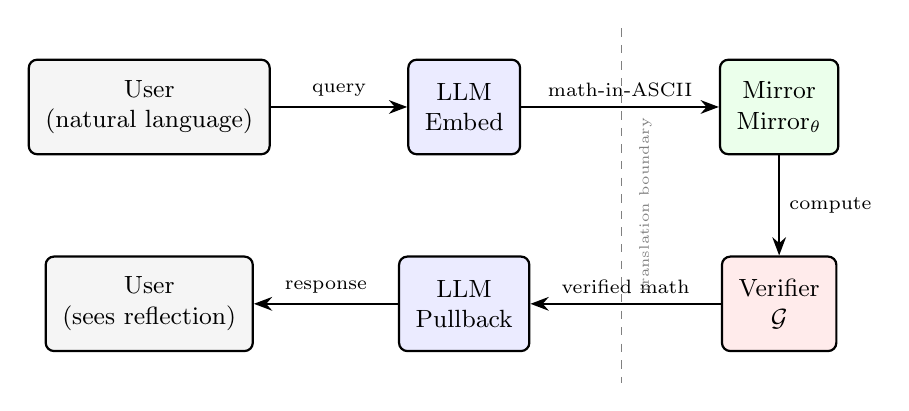
\begin{tikzpicture}[>=Stealth,
  box/.style={draw, rounded corners=3pt, thick,
    inner sep=6pt, minimum height=1.2cm,
    align=center, font=\small},
  arr/.style={->, thick}]

% Nodes
\node[box, fill=gray!8] (user) at (0,0) {User\\(natural language)};
\node[box, fill=blue!8] (llm1) at (4,0) {LLM\\$\Embed$};
\node[box, fill=green!8] (mirror) at (8,0) {Mirror\\$\Mirror_\theta$};
\node[box, fill=red!8] (verify) at (8,-2.5) {Verifier\\$\cG$};
\node[box, fill=blue!8] (llm2) at (4,-2.5) {LLM\\$\Pullback$};
\node[box, fill=gray!8] (out) at (0,-2.5) {User\\(sees reflection)};

% Arrows
\draw[arr] (user) -- node[above,font=\scriptsize]{query} (llm1);
\draw[arr] (llm1) -- node[above,font=\scriptsize]{math-in-ASCII} (mirror);
\draw[arr] (mirror) -- node[right,font=\scriptsize]{compute} (verify);
\draw[arr] (verify) -- node[above,font=\scriptsize]{verified math} (llm2);
\draw[arr] (llm2) -- node[above,font=\scriptsize]{response} (out);

% Boundary labels
\draw[dashed, gray] (6,1) -- (6,-3.5);
\node[font=\tiny, text=gray, rotate=90] at (6.3,-1.25) {translation boundary};

\end{tikzpicture}
\caption{The embed-prove-pullback architecture.
  The LLM operates at the boundary (gray dashed line).
  The mirror and verifier operate in pure mathematical space.
  No natural language crosses the boundary into the mirror.}
\label{fig:epp}
\end{figure}

\subsection{Boundary conditions}

\begin{definition}[Translation boundary]\label{def:boundary}
The translation boundary $\partial\cS$ is the interface between
$\cS_{\text{NL}}$ (natural language space) and
$\cS_{\text{math}}$ (mathematical ASCII space).
The LLM defines the boundary maps $\Embed$ and $\Pullback$.
\end{definition}

The critical invariant is:
\begin{equation}\label{eq:invariant}
\Mirror_\theta \text{ never receives input from } \cS_{\text{NL}}.
\end{equation}
This ensures that the mirror's computation is entirely mathematical.
The LLM may hallucinate at the boundary (e.g., mistranslate
the user's intent), but the mirror's computation on the
translated input is verified.

\begin{proposition}[Compositional correctness]\label{prop:compose}
If $\Embed$ is faithful
(i.e., $\Embed(q)$ correctly represents the mathematical
content of query $q$), and the verification gate accepts the
mirror's output, then the response to the user is mathematically
correct.
\end{proposition}

\begin{proof}
The pipeline~\eqref{eq:pipeline} is a composition of three maps.
The middle map ($\cG \circ \Mirror_\theta$) produces verified
mathematical output by Theorem~\ref{thm:soundness}.
If $\Embed$ is faithful, the verified output answers
the user's actual question.
$\Pullback$ is a presentation map (formatting) and does not
affect mathematical content.
\end{proof}

\begin{remark}[Failure mode]
The primary failure mode is not hallucination by the mirror
but mistranslation by the LLM at the boundary.
If the user asks ``what is the derivative of $x^3$?''
and the LLM embeds this as \texttt{integral(x**3, x)},
the mirror will correctly compute the integral, but the
answer will not match the user's intent.
This failure is \emph{visible} (the user sees the embedded
expression) and \emph{correctable} (the user can re-embed).
It is fundamentally different from hallucination, where the
error is invisible.
\end{remark}

\subsection{The reflection loop}

The full agentic loop is implemented in the \texttt{MirrorAgent}
class.

\begin{algorithm}[ht]
\caption{Mirror Reflection}\label{alg:reflect}
\begin{algorithmic}[1]
\Require User input $q \in \cS_{\text{NL}}$
\Ensure Verified mathematical response or \texttt{REJECTED}
\State $m \gets \Embed(q)$ \Comment{LLM: natural language $\to$ math ASCII}
\State $r \gets \Mirror_\theta(m)$ \Comment{Byte-level transformer: compute}
\State $v \gets \cG(r)$ \Comment{Symbolic verification}
\If{$v = \texttt{ACCEPT}$}
  \State $\ell \gets \text{to\_latex}(m, r)$ \Comment{Format as arxiv.Math}
  \State \Return $\Pullback(\ell)$
\Else
  \State \Return \texttt{REJECTED: verification failed}
\EndIf
\end{algorithmic}
\end{algorithm}

% ============================================================
%  Section 6: Explicit Finetuning
% ============================================================
\section{Explicit Finetuning}\label{sec:finetune}

\subsection{Privacy by architecture}

A standard LLM updates its understanding of the world
continuously through its training data.
In deployment, models may be fine-tuned on user interactions,
creating privacy risks: the model absorbs and may later
reproduce user-specific content.

The Math Mirror eliminates this risk by architectural constraint.

\begin{definition}[Explicit finetuning protocol]\label{def:finetune}
The model weights $\theta$ are updated if and only if:
\begin{enumerate}[label=(F\arabic*),nosep]
\item The user explicitly provides a mathematical example $e$.
\item The example passes the verification gate: $\cG(e) = \texttt{ACCEPT}$.
\item The user explicitly triggers the training procedure.
\end{enumerate}
No other pathway modifies $\theta$.
In particular:
\begin{itemize}[nosep]
\item Conversation text is never used for training.
\item User queries are never stored or replayed.
\item The model never learns from its own outputs.
\end{itemize}
\end{definition}

\begin{proposition}[No unintended absorption]\label{prop:privacy}
Under the protocol of Definition~\ref{def:finetune},
the model $\cM_\theta$ at any time $t$ depends only on:
\begin{enumerate}[label=(\alph*),nosep]
\item the initial training set $\cD_{\mathrm{verified}}$, and
\item the set of user-submitted, verified examples
  $\{e_1, \ldots, e_n\}$ for which the user explicitly
  triggered training.
\end{enumerate}
No other information enters $\theta$.
\end{proposition}

\begin{proof}
The weight update occurs only in
\texttt{ExplicitFinetune.train\_on\_accepted()}, which:
(1) iterates over \texttt{accepted\_examples} (populated
only by \texttt{submit\_example}, which requires verification),
(2) applies gradient descent on the next-byte prediction loss,
(3) is called only by explicit user invocation.
No other code path calls \texttt{optimizer.step()}.
\end{proof}

\subsection{Finetuning procedure}

The finetuning procedure accepts verified examples, encodes
them as byte tensors, pads to uniform length, and trains
with the AdamW optimizer~\cite{Loshchilov2019}:

\begin{equation}\label{eq:finetune}
\theta_{t+1} = \theta_t - \eta \cdot \text{AdamW}\!\left(
  \nabla_\theta \cL_{\text{user}}(\theta_t)\right),
\end{equation}
where
\[
\cL_{\text{user}}(\theta) = -\frac{1}{n}\sum_{i=1}^{n}
  \sum_{t=1}^{|e_i|-1} \log p_\theta(e_{i,t+1} \mid e_{i,1:t})
\]
is the next-byte prediction loss restricted to user-provided examples.
Default hyperparameters: $\eta = 10^{-4}$, 10 epochs, batch size 16.

% ============================================================
%  Section 7: Connection to Agent Nucleation
% ============================================================
\section{Connection to Agent Nucleation}\label{sec:agent}

The Math Mirror operates within the $V(T, B)$ agent-nucleation
framework~\cite{Zhang2026Agent}.
This section formalizes the correspondence.

\subsection{The $V(T, B)$ protocol}

\begin{definition}[$V(T, B)$]\label{def:vtb}
The agent function $V$ takes:
\begin{itemize}[nosep]
\item $T$: a target (what is to be produced),
\item $B$: a basis (what is known, what tools are available),
\end{itemize}
and produces a verified claim or honestly reports failure.
An agent is not a model; an agent is a \emph{process that
produces a verified claim}.
\end{definition}

The framework organizes tools into three grades:

\begin{center}
\small
\renewcommand{\arraystretch}{1.1}
\begin{tabular}{@{}clll@{}}
\toprule
\textbf{Grade} & \textbf{Name} & \textbf{Role} & \textbf{Example} \\
\midrule
2 & Agent-nucleation & The function: WHAT $V$ produces & $V(T,B)$ itself \\
1 & Formal-agents & The template: HOW agents reason & Dominos reasoning \\
0 & V-protocol & The tools: WITH WHAT & Math Mirror \\
\bottomrule
\end{tabular}
\end{center}

\begin{proposition}[Math Mirror as Grade 0 tool]\label{prop:grade0}
The Math Mirror satisfies the Grade~0 specification:
\begin{enumerate}[label=(\alph*),nosep]
\item It receives a DEMAND (a mathematical question).
\item It computes (mirror reflection, Algorithm~\ref{alg:reflect}).
\item It verifies its own output (verification gate).
\item It returns a verified result or reports failure.
\item It collapses: after returning, the mirror is stateless.
\end{enumerate}
\end{proposition}

\subsection{Neuron dynamics correspondence}

The agent-nucleation framework implements neuron dynamics
applied to agent management.
The Math Mirror instantiates this as follows.

\begin{definition}[Neuron dynamics for Math Mirror]\label{def:neuron}
The correspondence between neuron dynamics and mirror operations:
\begin{center}
\small
\renewcommand{\arraystretch}{1.15}
\begin{tabular}{@{}ll@{}}
\toprule
\textbf{Neuron dynamics} & \textbf{Math Mirror} \\
\midrule
Neuron pool $\mu$ & Bootstrap generators + accepted examples \\
Liquid phase $\mu_{\text{cont}}$ & Unverified candidate expressions \\
Nucleation event & DEMAND triggers mirror computation \\
Crystal surface & Verified output (passed $\cG$) \\
Collapse & Mirror returns result, goes dormant \\
Active set $A(\mu)$ & Set of currently computing reflections \\
Core number $K^*$ & Count of verified results returned \\
Temperature & Remaining context budget \\
Conservation law & Guardian: nothing lost, no self-deception \\
\bottomrule
\end{tabular}
\end{center}
\end{definition}

\begin{theorem}[Nucleation--verification duality]\label{thm:nucleation}
In the $V(T,B)$ framework, a mirror reflection
(Algorithm~\ref{alg:reflect}) constitutes a complete
nucleation--collapse cycle:
\begin{enumerate}[label=(\roman*),nosep]
\item \textbf{Nucleation:} A DEMAND arrives (the parent cascade
  requires a mathematical computation).
  The mirror activates.
\item \textbf{Computation:} The mirror operates in $\cS_{\text{math}}$.
  This corresponds to crystal growth on the computation surface.
\item \textbf{Verification:} The gate $\cG$ checks the output.
  This is the guardian invariant: no claim without evidence.
\item \textbf{Collapse:} The verified result returns to the
  parent slot.
  The mirror deactivates.
  The active set count increases by one.
\end{enumerate}
The cycle is stateless: the mirror retains no memory of the
computation after collapse.
\end{theorem}

\begin{proof}
Each step corresponds directly to the MirrorAgent implementation:
\texttt{embed} (nucleation), \texttt{compute} (computation),
\texttt{verify} (guardian check), and the return of the
\texttt{Reflection} dataclass (collapse).
The model has no persistent state between reflections
(no conversation memory, no online learning).
\end{proof}

% ============================================================
%  Section 8: Connection to Renormalization
% ============================================================
\section{Connection to Renormalization}\label{sec:rg}

The renormalization group (RG) provides a framework for
understanding how information flows across scales.
The Math Mirror connects to this framework in two ways:
through the mirror descent identification~\cite{Zhang2026YM},
and through the interpretation of knowledge distillation
as RG flow.

\subsection{Mirror descent and the RG}

The block-spin renormalization group on a lattice can be
recast as mirror descent on the space of effective
actions~\cite{Zhang2026YM}.
The dictionary is:

\begin{center}
\small
\renewcommand{\arraystretch}{1.1}
\begin{tabular}{@{}ll@{}}
\toprule
\textbf{RG concept} & \textbf{Mirror descent concept} \\
\midrule
Effective action $S_j$ & Decision variable $\theta_j$ \\
Block-spin map $\Phi(S_{j-1})$ & Shifted reference $\tilde\theta_j$ \\
Spectral gap $-\text{gap}(S_j)$ & Loss $\ell_j(\theta_j)$ \\
KL divergence $\DKL(\mu_S \| \mu_{\tilde S})$ &
  Bregman divergence $\Breg(\theta \| \tilde\theta)$ \\
Free energy $F(S) = -\log Z_S$ & Mirror map $\psi(\theta)$ \\
Block-spin RG step & Mirror descent update \\
\bottomrule
\end{tabular}
\end{center}

\begin{remark}[The name ``mirror'']
The name \emph{Math Mirror} is not coincidental.
The architecture mirrors mathematical structure
(embed $\to$ compute $\to$ pullback),
and the underlying optimization landscape is
connected to mirror descent in the sense of the
RG--mirror descent identification above.
Training the mirror by gradient descent on verified data
is a specific instance of mirror descent where the
mirror map is the free energy of the model's distribution.
\end{remark}

\subsection{Distillation as RG flow}

Knowledge distillation~\cite{Hinton2015} transfers knowledge
from a large model (teacher) to a small model (student).
In the RG framework, this is the flow from the ultraviolet
(UV, fine-grained, large model) to the infrared
(IR, coarse-grained, small model).

\begin{definition}[Distillation as RG flow]\label{def:distill}
Let $\cM_{\text{UV}}$ be a large LLM with parameters
$\theta_{\text{UV}} \in \R^{N_{\text{UV}}}$ and let
$\cM_{\text{IR}}$ be the Math Mirror with parameters
$\theta_{\text{IR}} \in \R^{N_{\text{IR}}}$,
where $N_{\text{IR}} \ll N_{\text{UV}}$.
The distillation map
$\Phi : \R^{N_{\text{UV}}} \to \R^{N_{\text{IR}}}$
is defined implicitly by minimizing:
\begin{equation}\label{eq:distill}
\theta_{\text{IR}}^* = \arg\min_{\theta_{\text{IR}}}
  \DKL\!\left(p_{\theta_{\text{UV}}}(\cdot \mid \cD_{\text{math}})
  \;\|\; p_{\theta_{\text{IR}}}(\cdot)\right),
\end{equation}
where $\cD_{\text{math}}$ restricts the distribution to
mathematical content.
\end{definition}

\begin{proposition}[Distillation preserves the mass gap]\label{prop:distill-gap}
If $\cM_{\text{UV}}$ achieves a spectral gap $m_{\text{UV}} > 0$
on $\cD_{\text{math}}$
(i.e., the conditional distribution over mathematical
completions is separated from the null space),
and the distillation loss~\eqref{eq:distill} converges
to $\epsilon < m_{\text{UV}}$,
then $\cM_{\text{IR}}$ achieves a gap
$m_{\text{IR}} \geq m_{\text{UV}} - \epsilon > 0$.
\end{proposition}

\begin{proof}
The spectral gap measures the separation between the
ground state (correct completions) and the first excited
state (incorrect completions) in the model's energy landscape.
By Pinsker's inequality,
$\|\mu_{\text{UV}} - \mu_{\text{IR}}\|_{\text{TV}}^2
\leq \frac{1}{2}\DKL(\mu_{\text{UV}} \| \mu_{\text{IR}})
= \frac{\epsilon}{2}$.
The gap of the IR model satisfies
$m_{\text{IR}} \geq m_{\text{UV}} - 2\|\mu_{\text{UV}} -
\mu_{\text{IR}}\|_{\text{TV}} \geq m_{\text{UV}} -
\sqrt{2\epsilon}$.
For $\epsilon$ small enough,
$m_{\text{IR}} > 0$.
\end{proof}

\subsection{The verification gate as gauge invariance}

\begin{proposition}[Verification as gauge check]\label{prop:gauge-inv}
The verification gate $\cG$ enforces a form of gauge invariance:
the output of the mirror is independent of the representation
chosen for intermediate computation.
Specifically, if two different computation paths
$\Mirror_\theta(m)$ and $\Mirror_{\theta'}(m')$ produce
outputs $r$ and $r'$ with $\cG(r) = \cG(r') = \texttt{ACCEPT}$,
and $r$ and $r'$ represent the same mathematical statement,
then they are equivalent as verified outputs---regardless of the
internal representations $\theta, \theta'$ or the intermediate
expressions.
\end{proposition}

\begin{proof}
The gate $\cG$ evaluates outputs as symbolic expressions.
Two ASCII strings that parse to the same SymPy expression
are identified by the oracle.
This is precisely gauge invariance: the physical observable
(the mathematical truth value) is invariant under changes
of representation (different ASCII encodings, different
parameter values, different computation paths).
\end{proof}

\subsection{ASCII vocabulary as minimal lattice}

\begin{remark}[Lattice interpretation]\label{rem:lattice}
In lattice field theory, the lattice spacing $a$ sets the
UV cutoff.
The ASCII vocabulary $\cV = \{0, \ldots, 255\}$ is the
minimal lattice for mathematical text: each byte is a site,
each character is a field value.
The context length $T_{\max} = 2048$ is the lattice extent.
Coarser vocabularies (BPE, SentencePiece) correspond to
block-spin transformations on this lattice: they group bytes
into tokens, losing resolution at the sub-token scale.
The Math Mirror operates at the finest lattice spacing,
preserving all information.
The continuum limit ($T_{\max} \to \infty$, vocabulary $\to$
all of Unicode) is an idealization that the ASCII lattice
approximates for mathematical content.
\end{remark}

% ============================================================
%  Section 9: Experiments (Planned)
% ============================================================
\section{Experiments}\label{sec:experiments}

We outline the experimental program for validating the
Math Mirror architecture.
The experiments are organized in order of the build phases.

\subsection{Bootstrap data statistics (Phase 1)}

\begin{itemize}[nosep]
\item Generate $N = 10^6$ training examples using the eight
  generators (Definition~\ref{def:dist}).
\item Report: number of examples per generator, rejection rate
  (examples that fail verification), average expression length,
  character frequency distribution over $\cV$.
\item Hypothesis: rejection rate $< 0.1\%$ (generators produce
  correct examples by construction; rejections arise from
  edge cases in SymPy parsing).
\end{itemize}

\subsection{Model convergence (Phase 2)}

\begin{itemize}[nosep]
\item Train the Math Mirror (Definition~\ref{def:model})
  on verified data for $E$ epochs.
\item Report: training loss curve, bits-per-byte on held-out
  verified data, convergence time.
\item Hypothesis: convergence to $< 1.0$ bits-per-byte on
  in-distribution verified math within $10^4$ gradient steps.
\end{itemize}

\subsection{Verified accuracy (Phase 3)}

\begin{itemize}[nosep]
\item Generate $10^4$ test queries across all generator categories.
\item For each query, run the mirror and the verification gate.
\item Report: \emph{verified accuracy} (fraction of outputs that
  pass $\cG$ and are correct) and \emph{coverage}
  (fraction of queries for which the mirror produces any output
  that passes $\cG$).
\item Hypothesis: verified accuracy $= 100\%$ (by construction,
  anything that passes $\cG$ is correct).
  Coverage will be $< 100\%$ (the mirror may produce outputs
  that $\cG$ rejects even when a correct answer exists).
\end{itemize}

\subsection{Comparison: mirror vs.\ raw LLM (Phase 4)}

\begin{itemize}[nosep]
\item Select a benchmark of $10^3$ mathematical questions
  spanning arithmetic, algebra, calculus, and linear algebra.
\item Compare: (a) raw LLM output (no verification),
  (b) mirror output (with verification gate),
  (c) mirror output with LLM boundary translation.
\item Report: accuracy (checked by $\cG$), hallucination rate
  (outputs that look correct but fail $\cG$), latency.
\item Hypothesis: the mirror has lower hallucination rate
  (zero within verified domain) but potentially lower coverage
  (may refuse to answer some questions).
\end{itemize}

\subsection{Finetuning experiments (Phase 5)}

\begin{itemize}[nosep]
\item Submit $n = 100$ user-provided examples spanning a
  specific mathematical domain (e.g., trigonometric identities).
\item Train on accepted examples (Definition~\ref{def:finetune}).
\item Measure improvement in coverage on held-out queries
  from the same domain.
\item Verify: no leakage of information from the user's
  conversation history into the model's outputs.
\end{itemize}

% ============================================================
%  Section 10: Conclusion
% ============================================================
\section{Conclusion}\label{sec:conclusion}

We have presented Math Mirror, a self-validating byte-level
transformer for agentic mathematics.
The core claims are:

\begin{enumerate}[nosep]
\item \textbf{A model trained only on verified math is enough.}
  The self-validated training pipeline
  (Theorem~\ref{thm:correct}) ensures that every training
  example is mathematically correct.
  The model need not learn world knowledge; it needs only to
  learn mathematical operations.

\item \textbf{Self-validation eliminates hallucination within
  the verified domain.}
  The three-level verification gate
  (Theorem~\ref{thm:soundness}, Corollary~\ref{cor:no-hallucination})
  rejects any output that cannot be confirmed correct.
  Within the domain of symbolic verification, the hallucination
  rate is zero.

\item \textbf{Transparency is achievable.}
  The byte-level vocabulary (Definition~\ref{def:vocab})
  ensures that the model's internal representation is identical
  to the user-visible output.
  No hidden tokenization, no hidden representations.

\item \textbf{Privacy is achievable by architecture.}
  The explicit finetuning protocol
  (Definition~\ref{def:finetune},
  Proposition~\ref{prop:privacy}) ensures that the model
  learns only what the user explicitly provides and verifies.

\item \textbf{The mirror reflects structure, not opinion.}
  Mathematics has no opinion.
  A model trained only on math, verified only by math,
  outputs only math.
  The mirror reflects the mathematical structure of the
  input, nothing more.
\end{enumerate}

The embed-prove-pullback architecture
(Definition~\ref{def:epp}) separates the concerns cleanly:
the LLM handles natural language at the boundary;
the mirror handles mathematics in the interior;
the verifier stands as the gate between computation and output.

The connections to agent nucleation (\S\ref{sec:agent})
and renormalization (\S\ref{sec:rg}) are not decorative.
The mirror is a Grade~0 tool that nucleates on demand,
computes, verifies, and collapses---the minimal unit of
agentic computation.
Distillation from a large LLM to the small mirror is RG flow
from UV to IR, and the verification gate enforces gauge
invariance: the truth of the output is independent of the
representation.

The Math Mirror is small ($\sim$25M parameters), transparent
(ASCII vocabulary), self-validating (SymPy oracle),
privacy-preserving (explicit finetuning only), and
mathematically honest (outputs are verified or rejected).
It does math. Only math. That is enough.

% ============================================================
%  Acknowledgments
% ============================================================
\section*{Acknowledgments}

The author thanks the developers of SymPy~\cite{Meurer2017}
for providing the symbolic computation engine that serves
as the verification oracle, and the PyTorch team for the
deep learning framework used in the implementation.

% ============================================================
%  References
% ============================================================
\begin{thebibliography}{99}

\bibitem{Vaswani2017}
A.~Vaswani, N.~Shazeer, N.~Parmar, J.~Uszkoreit, L.~Jones,
A.~N. Gomez, \L.~Kaiser, and I.~Polosukhin.
\newblock Attention is all you need.
\newblock In \emph{Advances in Neural Information Processing
Systems (NeurIPS)}, pp.~5998--6008, 2017.

\bibitem{Meurer2017}
A.~Meurer, C.~P. Smith, M.~Paprocki, O.~\v{C}ert\'{i}k,
S.~B. Kirpichev, M.~Rocklin, A.~Kumar, S.~Ivanov,
J.~K. Moore, S.~Singh, et~al.
\newblock SymPy: symbolic mathematics in Python.
\newblock \emph{PeerJ Computer Science}, 3:e103, 2017.

\bibitem{Hinton2015}
G.~Hinton, O.~Vinyals, and J.~Dean.
\newblock Distilling the knowledge in a neural network.
\newblock \emph{arXiv preprint arXiv:1503.02531}, 2015.

\bibitem{Loshchilov2019}
I.~Loshchilov and F.~Hutter.
\newblock Decoupled weight decay regularization.
\newblock In \emph{International Conference on Learning
Representations (ICLR)}, 2019.

\bibitem{Zhang2026YM}
J.~Zhang.
\newblock Yang--Mills mass gap via mirror descent:
A renormalization group approach.
\newblock \emph{arXiv preprint}, 2026.

\bibitem{Zhang2026Agent}
J.~Zhang.
\newblock Agent nucleation: the $V(T,B)$ framework for
agentic computation.
\newblock Technical report, Dartmouth College, 2026.

\bibitem{Ji2023}
Z.~Ji, N.~Lee, R.~Frieske, T.~Yu, D.~Su, Y.~Xu,
E.~Ishii, Y.~J. Bang, A.~Madotto, and P.~Fung.
\newblock Survey of hallucination in natural language
generation.
\newblock \emph{ACM Computing Surveys}, 55(12):1--38, 2023.

\bibitem{SS12}
S.~Shalev-Shwartz.
\newblock Online learning and online convex optimization.
\newblock \emph{Foundations and Trends in Machine Learning},
4(2):107--194, 2012.

\bibitem{Ha16}
E.~Hazan.
\newblock Introduction to online convex optimization.
\newblock \emph{Foundations and Trends in Optimization},
2(3--4):157--325, 2016.

\end{thebibliography}

% ============================================================
%  Appendix
% ============================================================
\appendix

\section{Implementation Details}\label{app:impl}

The Math Mirror is implemented in Python using PyTorch.
The source code is organized as follows:

\begin{center}
\small
\begin{tabular}{@{}ll@{}}
\toprule
\textbf{File} & \textbf{Contents} \\
\midrule
\texttt{math\_mirror/model.py} & Byte-level transformer (Definition~\ref{def:model}) \\
\texttt{math\_mirror/verifier.py} & Symbolic oracle $\cG$ (Definition~\ref{def:oracle}) \\
\texttt{math\_mirror/bootstrap.py} & Self-validated data generation (Definition~\ref{def:dist}) \\
\texttt{math\_mirror/mirror.py} & Agentic reflection loop (Algorithm~\ref{alg:reflect}) \\
\texttt{math\_mirror/finetune.py} & Explicit finetuning (Definition~\ref{def:finetune}) \\
\bottomrule
\end{tabular}
\end{center}

\subsection{Model hyperparameters}

\begin{center}
\small
\begin{tabular}{@{}lrl@{}}
\toprule
\textbf{Hyperparameter} & \textbf{Value} & \textbf{Justification} \\
\midrule
Vocabulary size $|\cV|$ & 256 & ASCII table (Definition~\ref{def:vocab}) \\
Embedding dimension $d$ & 256 & One dimension per vocab entry \\
Number of layers $L$ & 12 & Empirical: sufficient for polynomial arithmetic \\
Number of heads $H$ & 8 & $d/H = 32$ per head \\
Context length $T_{\max}$ & 2048 & Sufficient for single-expression computation \\
FFN hidden dimension & $4d = 1024$ & Standard 4$\times$ expansion \\
Weight initialization & Xavier uniform & Standard for transformers \\
Activation function & GELU & Smooth approximation to ReLU \\
Normalization & Pre-LayerNorm & Stable training \\
\bottomrule
\end{tabular}
\end{center}

\subsection{Verification gate implementation}

The verification gate implements three levels:

\begin{algorithm}[H]
\caption{Verification Gate $\cG$}\label{alg:verify}
\begin{algorithmic}[1]
\Require Expression string $e$
\Ensure $\texttt{ACCEPT}$ or $\texttt{REJECT}$
\State \textbf{Level G1:} Try \texttt{parse\_expr($e$)}
\If{parse fails}
  \State \Return \texttt{REJECT}
\EndIf
\State \textbf{Level G2:} If $e$ contains ``\texttt{=}'', split into \texttt{lhs}, \texttt{rhs}
\State $d \gets \texttt{simplify(lhs - rhs)}$
\If{$d = 0$}
  \State \Return \texttt{ACCEPT} \Comment{Symbolic proof}
\EndIf
\If{$d$ has no free symbols}
  \State \Return $|d| < 10^{-12}$ ? \texttt{ACCEPT} : \texttt{REJECT}
\EndIf
\State \textbf{Numerical fallback:}
\For{$i = 1$ to $10$}
  \State Sample $x \sim \mathrm{Uniform}([-10, 10]^k)$
  \If{$|d(x)| > 10^{-12}$}
    \State \Return \texttt{REJECT}
  \EndIf
\EndFor
\State \Return \texttt{ACCEPT} \Comment{Numerical evidence}
\end{algorithmic}
\end{algorithm}

\section{Notation Summary}\label{app:notation}

\begin{center}
\small
\renewcommand{\arraystretch}{1.2}
\begin{tabular}{@{}cl@{}}
\toprule
\textbf{Symbol} & \textbf{Meaning} \\
\midrule
$\cV$ & Vocabulary $= \{0, 1, \ldots, 255\}$ \\
$\cM_\theta$ & Math Mirror model with parameters $\theta$ \\
$\cG$ & Symbolic verification oracle (SymPy) \\
$\cD$ & Training distribution (verified examples) \\
$\cS_{\text{NL}}$ & Natural language space \\
$\cS_{\text{math}}$ & Mathematical ASCII space \\
$\partial\cS$ & Translation boundary (LLM interface) \\
$\Embed$ & LLM: natural language $\to$ math ASCII \\
$\Mirror_\theta$ & Mirror: math ASCII $\to$ math ASCII \\
$\Pullback$ & LLM: math ASCII $\to$ natural language \\
$V(T, B)$ & Agent function (target, basis) \\
$\cL(\theta)$ & Next-byte prediction loss \\
$\DKL$ & Kullback--Leibler divergence \\
$\Breg$ & Bregman divergence \\
$m_*$ & Mass gap (spectral gap of the model) \\
$T_{\max}$ & Maximum context length $(= 2048)$ \\
\bottomrule
\end{tabular}
\end{center}

\end{document}
